\section{Descripci�n de la Herramienta}

La Herramienta de Precios Chedraui busca precios
en tiendas de la competencia con el fin de igualar precios de productos en estas tiendas.
En general, la herramienta busca el precio m�s barato posible, 
o en su defecto el precio de mercado (moda nacional). 

Las tablas de datos son extraidas del mismo equipo 
donde corre la herramienta, no requiere de conexiones a bases de datos externas. 
La herramienta es capaz de correr en un cluster, las tablas de datos se extraen del mismo
en este caso de un Hadoop Filesystem (HDFS, Filesystem compartido por el cluster).

Los requerimientos f�sicos y de software se describen en la secci�n \ref{reqs},
la preparaci\'{o}n de los datos de entrada en la \ref{inputs},
las funciones de la herramienta y su uso en la \ref{funcions}, 
la descripci\'{o}n de los datos de salida en la \ref{outputs}. 
Finalmente, el proceso seguido por la herramienta se detalla en la secci�n \ref{process}, 
esta misma secci\'{o}n tiene una descripci\'{o}n poco t�cnica del proceso.

La Herramienta de Precios Chedraui corre sobre la consola de Spark,
la cu�l a su vez corre sobre la m�quina virtual de Java con el lenguaje Scala.
Opcionalmente, se puede utilizar el HDFS si se desea correr sobre un cluster.
La instalaci�n de las dependencias de la herramienta se cubre en la secci�n \ref{reqs}.
\begin{figure}[H]
	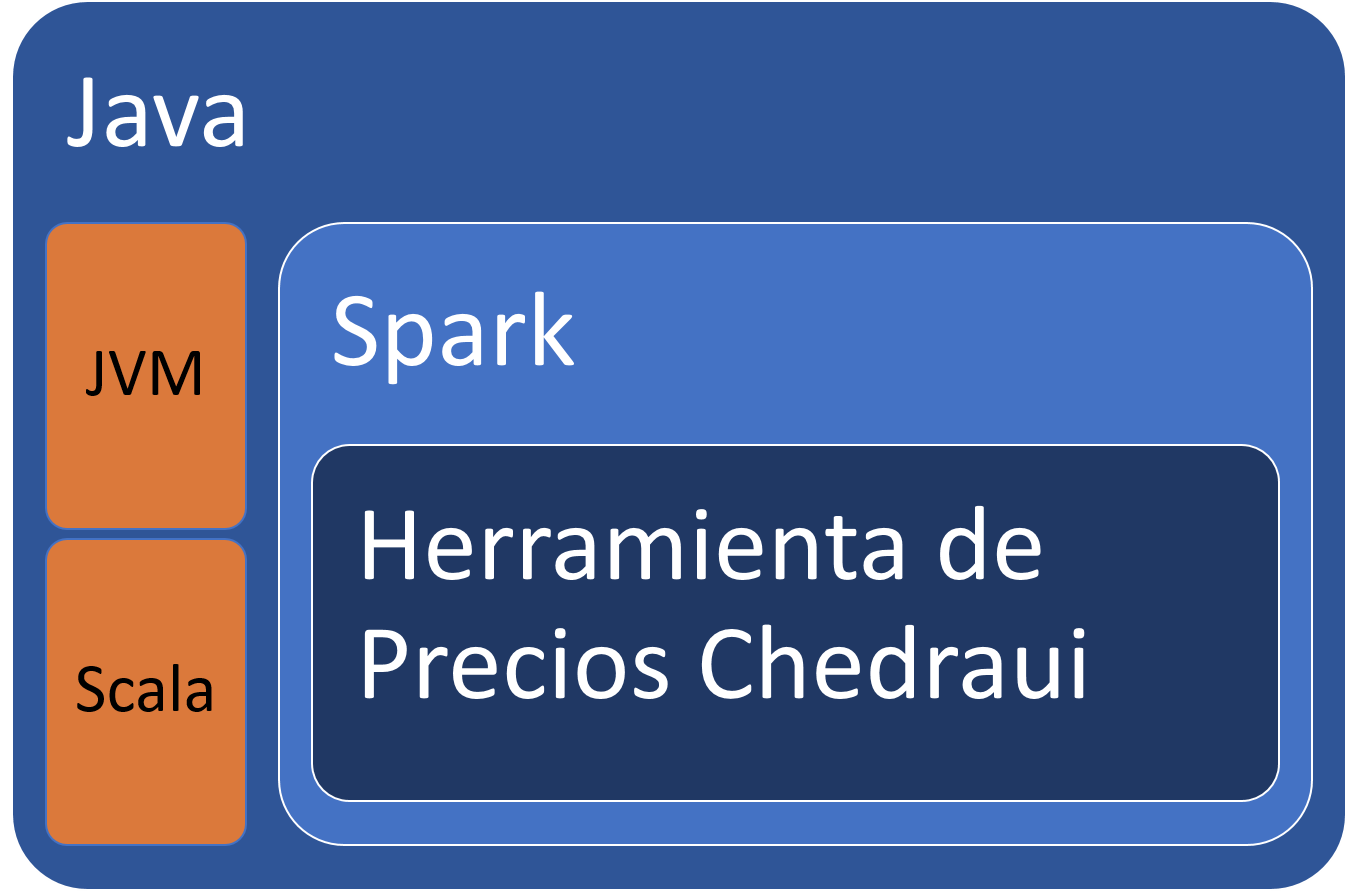
\includegraphics[scale=0.35]{diagDependencias}
	\centering
\end{figure}

En general, las funciones siguen el siguiente proceso: 
\begin{enumerate} 
\item El usuario coloca datos en la m�quina de trabajo.
\item El usuario hace una llamada a una funci�n de la herramienta.
\item La herramienta coloca resultados sobre una carpeta.
\end{enumerate}

\begin{figure}[H]
	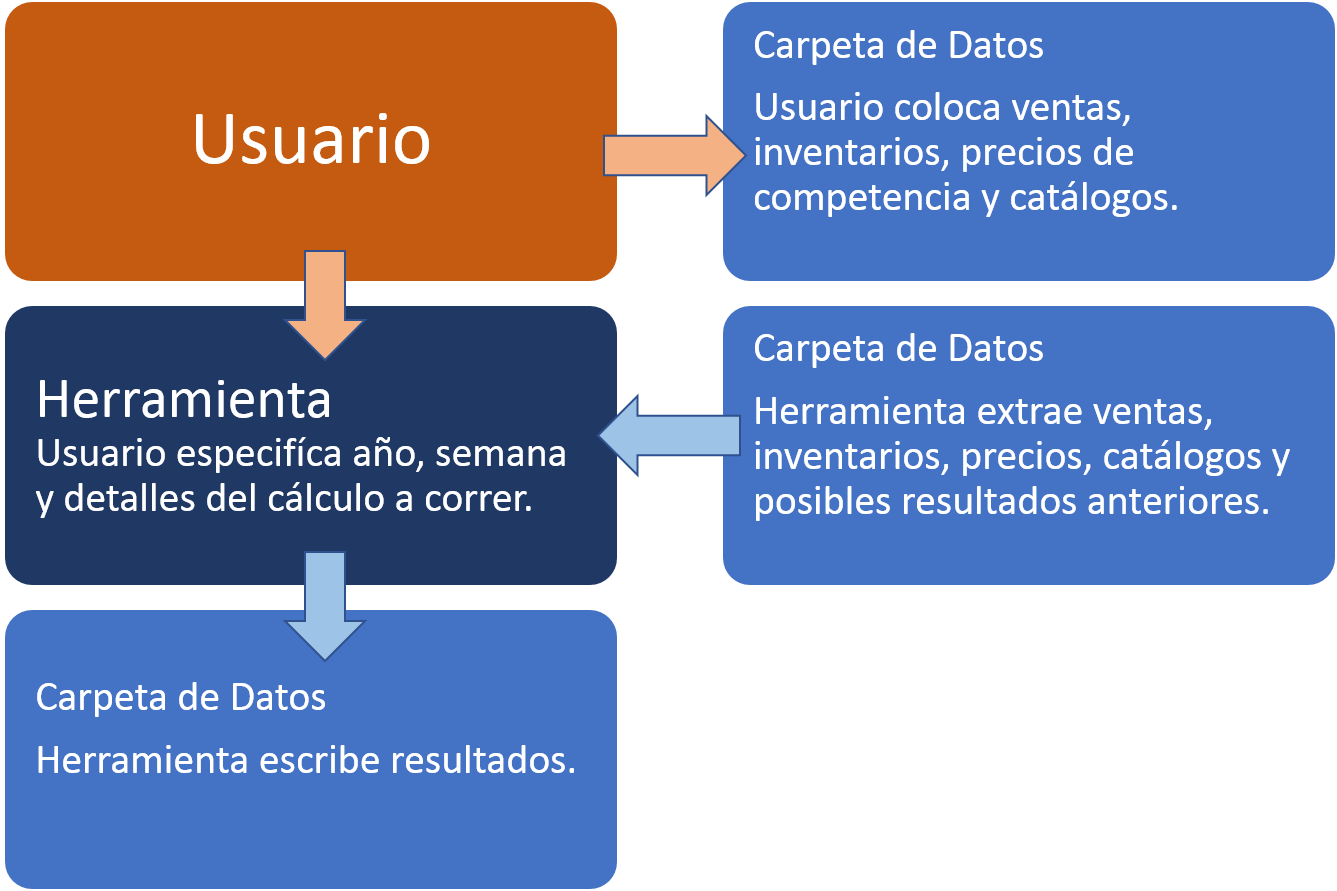
\includegraphics[scale=0.35]{diagProceso}
	\centering
\end{figure}



\subsection{Reglas de Negocio y Proceso}

A continuaci\'{o}n se detallan las reglas de negocio
utilizadas por la herramienta. 
El proceso principal la llevan a cabo cuatro funciones de la herramienta:
\begin{enumerate}
	\item calcCompetencia Preparaci\'{o}n de Precios de Competencia
	\item calcDatos Cruce de Precios y Detecci\'{o}n de Promociones
	\item calcPrecios Sugerencias de Precios
	\item calcImpactos C�lculo de Impactos de Cambio de Precio
\end{enumerate}



\subsubsection{Preparaci\'{o}n de Precios de Competencia}

La herramienta extraer� los precios de cada producto de la competencia a nivel UPC/Tienda, 
luego calcular� moda y mediana nacionales en la semana m�s reciente donde se haya encontrado cada UPC.
Adicionalmente, la herramienta calcular� la mediana 
de precio a lo largo de las semanas de un producto a nivel Tienda.

\subsubsection{Cruce de Precios y Detecci\'{o}n de Promociones}

La herramienta extraer� los inventarios y calcular� el precio de regulaci\'{o}n central:
\begin{equation}
P_{RC} = InvFinVta / InvFinUni
\end{equation}
A partir de las ventas (o del inventario seg�n especifique el usario) 
se cruzar� la matriz de competencia a nivel Tienda/Depto/SubDepto.
La matriz de competencia asocia Tiendas Chedraui a Tiendas de la competencia;
cada tienda de la competencia tiene un nivel de prioridad, 
donde la prioridad m�xima prioridad es 1 y la m�nima es 3.

Se cruzar�n los precios de la competencia. 
A nivel UPC/Tienda se tomar� el precio m�s reciente de la competencia,
a nivel UPC se toma la moda nacional m�s reciente 
y a nivel UPC/Tienda se toma la mediana de la Tienda a lo largo del tiempo.
Precios de cada producto ser�n marcados como promocionales 
si se cumple alguna de las siguientes condiciones:
\begin{equation}
\begin{aligned}
P &< P_{medianaTienda} (100-porcentaje) \\
P &< P_{modaNacional} (100-60)
\end{aligned}
\end{equation}
El porcentaje estar� especificado por un cat�logo cat\_promos. 
Un precio ser� marcado como remate si la condici\'{o}n anterior se cumple con porcentaje=60\%.



\subsubsection{Sugerencias de Precios}

Se obtiene el grupo de cada UPC de acuerdo al cat�logo cat\_grupos, 
posteriormente se calcula la moda nacional del grupo (el m�nimo de las modas nacionales de cada grupo)
y el precio de grupo a nivel tienda (el m�nimo de los precios de los productos del grupo a nivel tienda).

Por cada producto se calcula el precio sugerido de acuerdo a las siguientes reglas
aplicadas en orden:
\begin{enumerate}
\item El precio sugerido inicial por UPC es el precio de la competencia encontrado en 
las Tiendas de la competencia especificados en la matriz de competencia. 
\item Si no se ha encontrado precio o esta marcado como promocional/remate ser�
sustituido por la moda nacional. 
\item Si el precio sugerido es mayor al precio de grupo o no se ha encontrado un precio de competencia 
se sustituye el precio de grupo a nivel tienda.
\item Si el precio sugerido no ha sido encontrado se utiliza la moda de grupo. 
\item Se asocia a cada art�culo una excepci\'{o}n si 
al menos a un art�culo de su grupo se le da una excepci\'{o}n en el cat�logo de excepciones.
\end{enumerate}
Con estas reglas los �nicos productos que no presentan sugerencias de precios 
son aquellos que no se encuentran en las tablas de precios de la competencia.

Finalmente se pueden calcular los impactos que la regulaci\'{o}n de precios 
tiene sobre los precios Chedraui, esta �ltima funcionalidad la lleva a cabo la funci\'{o}n calcImpactos.
